%----------------------------------------------------------------------------------------
%	PACKAGES AND THEMES
%----------------------------------------------------------------------------------------

\documentclass{beamer}

\mode<presentation> {

% The Beamer class comes with a number of default slide themes
% which change the colors and layouts of slides. Below this is a list
% of all the themes, uncomment each in turn to see what they look like.

%\usetheme{default}
%\usetheme{AnnArbor}
%\usetheme{Antibes}
%\usetheme{Bergen}
%\usetheme{Berkeley}
%\usetheme{Berlin}
%\usetheme{Boadilla}
%\usetheme{CambridgeUS}
%\usetheme{Copenhagen}
%\usetheme{Darmstadt}
%\usetheme{Dresden}
%\usetheme{Frankfurt}
%\usetheme{Goettingen}
%\usetheme{Hannover}
%\usetheme{Ilmenau}
%\usetheme{JuanLesPins}
%\usetheme{Luebeck}
\usetheme{Madrid}
%\usetheme{Malmoe}
%\usetheme{Marburg}
%\usetheme{Montpellier}
%\usetheme{PaloAlto}
%\usetheme{Pittsburgh}
%\usetheme{Rochester}
%\usetheme{Singapore}
%\usetheme{Szeged}
%\usetheme{Warsaw}

% As well as themes, the Beamer class has a number of color themes
% for any slide theme. Uncomment each of these in turn to see how it
% changes the colors of your current slide theme.

%\usecolortheme{albatross}
%\usecolortheme{beaver}
%\usecolortheme{beetle}
%\usecolortheme{crane}
%\usecolortheme{dolphin}
%\usecolortheme{dove}
%\usecolortheme{fly}
%\usecolortheme{lily}
%\usecolortheme{orchid}
%\usecolortheme{rose}
%\usecolortheme{seagull}
%\usecolortheme{seahorse}
%\usecolortheme{whale}
%\usecolortheme{wolverine}

%\setbeamertemplate{footline} % To remove the footer line in all slides uncomment this line
%\setbeamertemplate{footline}[page number] % To replace the footer line in all slides with a simple slide count uncomment this line

%\setbeamertemplate{navigation symbols}{} % To remove the navigation symbols from the bottom of all slides uncomment this line
}

\usepackage{graphicx} % Allows including images
\usepackage{booktabs} % Allows the use of \toprule, \midrule and \bottomrule in tables
\usepackage{adjustbox}
\usepackage{tikz}
\usetikzlibrary{arrows.meta}
\tikzset{%
  >={Latex[width=2mm,length=2mm]},
  % Specifications for style of nodes:
            base/.style = {rectangle, rounded corners, draw=black,
                           minimum width=4cm, minimum height=1cm,
                           text centered, font=\sffamily},
  activityStarts/.style = {base, fill=blue!30},
       startstop/.style = {base, fill=red!30},
    activityRuns/.style = {base, fill=green!30},
         process/.style = {base, minimum width=2.5cm, fill=orange!15,
                           font=\ttfamily},
}
%----------------------------------------------------------------------------------------
%	TITLE PAGE
%----------------------------------------------------------------------------------------

\title[Viculum]{Konzept und Realisierung eines virtuellen Themenrundgangs der Fakultät Informatik zur Unterstützung bei der Studienwahl} % The short title appears at the bottom of every slide, the full title is only on the title page

\author{Prof. Dr. Jörg Röhrle} % Your name
\institute[HSALBSIG] % Your institution as it will appear on the bottom of every slide, may be shorthand to save space
{
Hochschule Albstadt-Sigamringen \\ % Your institution for the title page
\medskip
\textit{Domenico Milazzo (TI), milazzdo@hs-albsig.de} % Your email address
\newline
\textit{Maik Dürr (TI), duerrmai@hs-albsig.de} % Your email address
\newline
\textit{Fabian Altenberg (WIN), altenbfa@hs-albsig.de} % Your email address
\newline
}
\date{\today} % Date, can be changed to a custom date

\begin{document}

\begin{frame}
\titlepage % Print the title page as the first slide
\end{frame}

\begin{frame}
\frametitle{Überblick}
\begin{itemize}
\item Idee \& Features
\item Datenmodell
\item Datenzugriff
\item Live Demo \& Aussiechten
\end{itemize}
\end{frame}

%----------------------------------------------------------------------------------------
%	PRESENTATION SLIDES
%----------------------------------------------------------------------------------------

%------------------------------------------------

\begin{frame}
\frametitle{Idee \& Features}
Viculum ist ein virtuelles Curriculum um die Modulhandbücher jeder Veranstaltungen der Hochschule Albstadt-Sigmaringen mit verschiedensten Medien und einem dynamischen Zugriff aus einer Datenbank zu visualisieren.\\~\\

\begin{itemize}
\item Oracle Datenbank als Speichermedium
\item Unity als Visualisierung Tool der Virtual Reality
\item Dynamischen Aufbau der Szenen um Objekte
\item Bilder \& Video als zusätzliche Medien
\end{itemize}
\end{frame}

%------------------------------------------------

\begin{frame}
\frametitle{Datenbankmodell}
\begin{center}
\includegraphics[width=0.8\textwidth]{pictures/Datenmodell_Viculum.png}
\end{center}
\end{frame}


%------------------------------------------------

\begin{frame}
\frametitle{Datenzugriff}
\begin{adjustbox}{totalheight=\textheight-3\baselineskip}
\begin{columns}[c] % The "c" option specifies centered vertical alignment while the "t" option is used for top vertical alignment

\column{.45\textwidth} % Left column and width

\textbf{Ablauf}
\begin{enumerate}
\item Szenen starten und holt sich aus der Statischen Klasse die Informationen aus der vorherigen Szene.
\item leeres GameObjekt wird angestoßen und mit den Szenen Information gefüttert.
\item Das C\# Script des leeren GameObjekt wird ausgeführt.
\item Datenbankzugriff auf die Oracle Datenbank und deren Auswertung.
\item Die Informationen der Auswerten werden im Object angezeigt.
\end{enumerate}

\column{.3\textwidth} % Right column and width
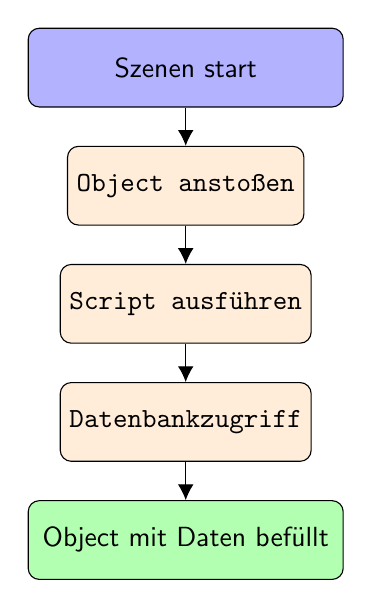
\begin{tikzpicture}[node distance=1.5cm,
    every node/.style={fill=white, font=\sffamily}, align=center]
  % Specification of nodes (position, etc.)
  \node (start)             [activityStarts]              	{Szenen start};
  \node (Object)     [process, below of=start]  {Object anstoßen};
  \node (Script)      [process, below of=Object]{Script ausführen};
  \node (DB)     [process, below of=Script]   		{Datenbankzugriff};
  \node (end)      [activityRuns, below of=DB]		{Object mit Daten befüllt};   
  % Specification of lines between nodes specified above
  % with aditional nodes for description 
  \draw[->]             (start) -- (Object);
  \draw[->]     		(Object) -- (Script);
  \draw[->]      		(Script) -- (DB);
  \draw[->]     		(DB) -- (end);
  \end{tikzpicture}


\end{columns}
\end{adjustbox}
\end{frame}

%------------------------------------------------

\begin{frame}
\Huge{\centerline{Demo}}
\end{frame}
\end{document} 